\documentclass[aspectratio=169, 10pt]{beamer}

% --- GÓI HỌC THUẬT & FONT TIẾNG VIỆT CHO XELATEX ---
\usepackage{fontspec}
\setmainfont{Arial}
\setsansfont{Arial}
\setmonofont{Consolas}

\usepackage{amsmath,amssymb}
\usepackage{graphicx}
\usepackage{booktabs}
\usepackage{tabularx}
\usepackage{multicol}
\usepackage{listings}
\usepackage{xcolor}
\usepackage{tikz}
\usetikzlibrary{shapes,arrows,positioning,fit,backgrounds,calc}
\usepackage{tcolorbox}
\tcbuselibrary{skins,breakable,listings}

% --- ĐỊNH NGHĨA MÀU SẮC CHUẨN ĐẠI HỌC & C# .NET ---
\definecolor{UniNavy}{RGB}{15, 44, 89}        % Xanh hải quân chủ đạo (#0F2C59)
\definecolor{UniBlue}{RGB}{29, 93, 155}       % Xanh Slate (#1D5D9B)
\definecolor{CSharpPurple}{RGB}{104, 33, 122} % Tím nhận diện C# & Visual Studio (#68217A)
\definecolor{UniLightBlue}{RGB}{232, 241, 252}% Nền xanh nhạt
\definecolor{UniOrange}{RGB}{225, 112, 18}    % Cam nhấn mạnh (#E17012)
\definecolor{UniGreen}{RGB}{30, 132, 73}      % Xanh lá thực hành (#1E8449)
\definecolor{UniDark}{RGB}{33, 37, 41}        % Màu chữ chính / nền console
\definecolor{CodeBg}{RGB}{248, 249, 250}      % Nền code
\definecolor{CSharpKeyword}{RGB}{0, 0, 255}   % Xanh dương từ khóa C#
\definecolor{CSharpString}{RGB}{163, 21, 21}  % Đỏ chuỗi C#
\definecolor{CSharpComment}{RGB}{0, 128, 0}   % Xanh lá chú thích C#

% --- CẤU HÌNH THEME BEAMER MADRID WIDESCREEN ---
\usetheme{Madrid}
\usecolortheme{whale}

\setbeamercolor{palette primary}{bg=UniNavy, fg=white}
\setbeamercolor{palette secondary}{bg=CSharpPurple, fg=white}
\setbeamercolor{palette tertiary}{bg=UniNavy!85, fg=white}
\setbeamercolor{palette quaternary}{bg=UniNavy, fg=white}

\setbeamercolor{structure}{fg=UniNavy}
\setbeamercolor{titlelike}{parent=structure, fg=UniNavy}
\setbeamercolor{frametitle}{bg=UniNavy, fg=white}
\setbeamercolor{frametitle continuation}{fg=white}
\setbeamercolor{normal text}{fg=UniDark}

% Cấu hình khối thông tin (Blocks)
\setbeamercolor{block title}{bg=UniBlue, fg=white}
\setbeamercolor{block body}{bg=UniLightBlue!40, fg=UniDark}
\setbeamercolor{block title example}{bg=UniGreen, fg=white}
\setbeamercolor{block body example}{bg=UniGreen!10, fg=UniDark}
\setbeamercolor{block title alerted}{bg=UniOrange, fg=white}
\setbeamercolor{block body alerted}{bg=UniOrange!10, fg=UniDark}

% Cấu hình Footline chuyên nghiệp
\setbeamertemplate{navigation symbols}{}
\setbeamertemplate{footline}{
  \leavevmode%
  \hbox{%
    \begin{beamercolorbox}[wd=.35\paperwidth,ht=2.5ex,dp=1.1ex,left,leftskip=2ex]{author in head/foot}%
      \usebeamerfont{author in head/foot}\textbf{Lớp IT26M} | Lập trình C\# \& .NET
    \end{beamercolorbox}%
    \begin{beamercolorbox}[wd=.45\paperwidth,ht=2.5ex,dp=1.1ex,center]{title in head/foot}%
      \usebeamerfont{title in head/foot}Chương 1: Introduction to Computers, Internet \& C\#
    \end{beamercolorbox}%
    \begin{beamercolorbox}[wd=.20\paperwidth,ht=2.5ex,dp=1.1ex,right,rightskip=2ex]{date in head/foot}%
      \usebeamerfont{date in head/foot}\insertframenumber{} / \inserttotalframenumber
    \end{beamercolorbox}%
  }%
  \vskip0pt%
}

% --- CẤU HÌNH GÓI LISTINGS CHO C# & TERMINAL ---
\lstdefinelanguage{CSharpCustom}{
  keywords={abstract, as, base, bool, break, byte, case, catch, char, checked, class, const, continue, decimal, default, delegate, do, double, else, enum, event, explicit, extern, false, finally, fixed, float, for, foreach, goto, if, implicit, in, int, interface, internal, is, lock, long, namespace, new, null, object, operator, out, override, params, private, protected, public, readonly, ref, return, sbyte, sealed, short, sizeof, stackalloc, static, string, struct, switch, this, throw, true, try, typeof, uint, ulong, unchecked, unsafe, ushort, using, virtual, void, volatile, while, async, await, var},
  keywordstyle=\color{CSharpKeyword}\bfseries,
  ndkeywords={Console, String, Math, Convert, Application, Form, GroupBox, RadioButton, Panel, Button, MouseEventArgs},
  ndkeywordstyle=\color{CSharpPurple}\bfseries,
  sensitive=true,
  comment=[l]{//},
  morecomment=[s]{/*}{*/},
  commentstyle=\color{CSharpComment}\itshape,
  stringstyle=\color{CSharpString},
  morestring=[b]",
  morestring=[b]'
}

\lstset{
  language=CSharpCustom,
  basicstyle=\ttfamily\scriptsize,
  numbers=left,
  numberstyle=\tiny\color{gray},
  stepnumber=1,
  numbersep=6pt,
  backgroundcolor=\color{CodeBg},
  frame=single,
  rulecolor=\color{black!20},
  tabsize=4,
  showstringspaces=false,
  breaklines=true,
  breakatwhitespace=true,
  columns=flexible,
  keepspaces=true,
  xleftmargin=12pt,
  framexleftmargin=10pt
}

% Style cho console output
\lstdefinestyle{terminalStyle}{
  basicstyle=\ttfamily\scriptsize\color{white},
  backgroundcolor=\color{UniDark},
  frame=single,
  rulecolor=\color{UniNavy},
  numbers=none,
  xleftmargin=6pt,
  framexleftmargin=6pt
}

% --- THÔNG TIN TRANG TIÊU ĐỀ ---
\title[\textbf{Lập trình C\# \& .NET -- Chương 1}]{\textbf{\LARGE KỸ THUẬT LẬP TRÌNH C\#}}
\subtitle{\textbf{\large Chương 1: Giới thiệu về Máy tính, Internet và Visual C\#}}
\author[\textbf{Khoa CNTT -- IT26M}]{\textbf{BÀI GIẢNG CHUẨN ĐẠI HỌC (3 TIẾT TÍCH HỢP)}\\Giáo trình: \textit{Visual C\# How to Program} (Deitel \& Deitel)}
\institute[\textbf{Lớp IT26M}]{\textbf{Khoa Công nghệ Thông tin -- Đại học Đông Á}\\\textbf{Đối tượng:} Lớp IT26M (Khóa 2026)}
\date[\textbf{2026}]{\textbf{Học kỳ I -- Năm học 2026}}

\begin{document}

% ==============================================================================
% SLIDE 1: TRANG TIÊU ĐỀ BÀI GIẢNG
% ==============================================================================
\begin{frame}[plain]
  \titlepage
  \begin{center}
    \scriptsize \color{gray} Bản quyền bài giảng thuộc Bộ môn Kỹ thuật Lập trình -- Phục vụ đào tạo Đại học chính quy
  \end{center}
\end{frame}

% ==============================================================================
% SLIDE 2: MỤC TIÊU BÀI HỌC & CHUẨN ĐẦU RA (CLOs)
% ==============================================================================
\begin{frame}{Mục tiêu Bài học \& Chuẩn đầu ra (CLOs)}
  \begin{block}{\textbf{Chuẩn đầu ra sinh viên cần đạt được sau buổi học 3 tiết:}}
    \begin{itemize}
      \item \textbf{CLO 1.1 (Understand):} Giải thích kiến trúc phần cứng, định luật Moore, 6 khối chức năng logic của máy tính và cấu trúc phân cấp dữ liệu từ Bit $\to$ Database $\to$ Big Data.
      \item \textbf{CLO 1.2 (Understand):} Nắm vững sự tiến hóa ngôn ngữ (Machine $\to$ Assembly $\to$ High-Level) và các trụ cột công nghệ đối tượng (Class, Object, Encapsulation, Inheritance).
      \item \textbf{CLO 1.3 (Apply):} Trình bày kiến trúc Microsoft .NET: Common Language Runtime (CLR), Managed Code, MSIL, JIT Compiler và tính độc lập nền tảng (.NET Core / .NET 8).
      \item \textbf{CLO 1.4 (Apply):} Sử dụng thành thạo môi trường Visual Studio IDE: Solution, Project, Form Designer, Toolbox, Properties Window và công cụ gỡ lỗi.
      \item \textbf{CLO 1.5 (Analyze / Create):} Vận dụng mô hình Lập trình trực quan và Hướng sự kiện (Event-Driven) để thực hành chạy thử (Test-Drive) và phân tích ứng dụng Painter.
    \end{itemize}
  \end{block}
  \vspace{-2mm}
  \begin{exampleblock}{\textbf{Phương pháp tiếp cận:}}
    Học tích hợp: \textbf{Lý thuyết chuyên sâu} kết hợp \textbf{3 bài Hands-on Labs} thực hành tại chỗ trên máy tính.
  \end{exampleblock}
\end{frame}

% ==============================================================================
% SLIDE 3: TIẾN TRÌNH BÀI HỌC 3 TIẾT
% ==============================================================================
\begin{frame}{Tiến trình Bài học 3 Tiết (150 Phút Tích hợp)}
  \begin{columns}[T]
    \begin{column}{0.32\textwidth}
      \begin{tcolorbox}[colback=UniNavy!5,colframe=UniNavy,title=\textbf{TIẾT 1 (50')},fonttitle=\small\bfseries]
        \textbf{Nền tảng \& Dữ liệu}
        \begin{itemize}\scriptsize
          \item Phần cứng vs Phần mềm
          \item Định luật Moore
          \item 6 khối logic máy tính
          \item Phân cấp dữ liệu
          \item Đo lường Byte (KB - YB)
          \item \textbf{[LAB 1]:} Khảo sát CPU, RAM \& Số nhị phân
        \end{itemize}
      \end{tcolorbox}
    \end{column}

    \begin{column}{0.32\textwidth}
      \begin{tcolorbox}[colback=CSharpPurple!5,colframe=CSharpPurple,title=\textbf{TIẾT 2 (50')},fonttitle=\small\bfseries]
        \textbf{OOP \& Kiến trúc .NET}
        \begin{itemize}\scriptsize
          \item Tiến hóa ngôn ngữ
          \item Compiler vs Interpreter
          \item Công nghệ đối tượng (OOP)
          \item Lịch sử ngôn ngữ C\#
          \item Nền tảng Microsoft .NET
          \item CLR, MSIL \& JIT Compiler
          \item \textbf{[LAB 2]:} Biên dịch CLI với .NET SDK
        \end{itemize}
      \end{tcolorbox}
    \end{column}

    \begin{column}{0.32\textwidth}
      \begin{tcolorbox}[colback=UniGreen!5,colframe=UniGreen,title=\textbf{TIẾT 3 (50')},fonttitle=\small\bfseries]
        \textbf{Visual Studio \& GUI Lab}
        \begin{itemize}\scriptsize
          \item Hệ điều hành Windows
          \item Visual Studio IDE
          \item Solution \& Projects
          \item Mô hình Event-Driven
          \item Khảo sát điều khiển GUI
          \item \textbf{[LAB 3]:} Test-Drive ứng dụng Painter
          \item Tổng kết \& Dặn dò
        \end{itemize}
      \end{tcolorbox}
    \end{column}
  \end{columns}
\end{frame}

% ==============================================================================
% SLIDE 4: TỔNG QUAN VỊ THẾ CỦA C# & .NET
% ==============================================================================
\begin{frame}{Tổng quan Vị thế của Ngôn ngữ C\# \& Nền tảng .NET}
  \begin{columns}[c]
    \begin{column}{0.55\textwidth}
      \begin{block}{\textbf{Vì sao chọn C\# cho Kỹ sư CNTT Khóa 2026?}}
        \begin{itemize}
          \item \textbf{Thanh lịch \& Hiện đại:} Được thiết kế bởi Anders Hejlsberg (cha đẻ Turbo Pascal, Delphi, TypeScript).
          \item \textbf{Mạnh mẽ \& Đa năng:} Hỗ trợ đa mô hình lập trình (OOP, Event-Driven, Functional, Generic, Async).
          \item \textbf{Hệ sinh thái khổng lồ:} Phát triển Web (ASP.NET Core), Desktop (WinForms, WPF, MAUI), Mobile (iOS/Android), Cloud (Azure) và Game (Unity 3D).
          \item \textbf{Hiệu năng vượt trội:} .NET 8 / .NET 9 đứng top đầu thế giới về tốc độ xử lý I/O và tối ưu bộ nhớ.
        \end{itemize}
      \end{block}
    \end{column}
    \begin{column}{0.42\textwidth}
      \begin{tcolorbox}[colback=UniLightBlue,colframe=UniBlue,title=\textbf{Triết lý Thiết kế C\#}]
        \centering
        \textbf{\Large "Powerful, Elegant, Safe \& Cross-Platform"}
        \vskip 2mm
        \scriptsize Kết hợp sức mạnh xử lý phần cứng của C++ với tính an toàn, năng suất phát triển siêu tốc của Java và Visual Basic.
      \end{tcolorbox}
    \end{column}
  \end{columns}
\end{frame}

% ==============================================================================
% SLIDE 5: TIẾT 1 TITLE
% ==============================================================================
\begin{frame}
  \vfill
  \centering
  \begin{beamercolorbox}[sep=8pt,center,shadow=true,rounded=true]{palette primary}
    \usebeamerfont{title}\Huge \textbf{TIẾT 1: NỀN TẢNG TÍNH TOÁN,}\\[2mm]
    \Large \textbf{TỔ CHỨC MÁY TÍNH \& PHÂN CẤP DỮ LIỆU}
  \end{beamercolorbox}
  \vfill
\end{frame}

% ==============================================================================
% SLIDE 6: 1.1 PHẦN CỨNG & PHẦN MỀM
% ==============================================================================
\begin{frame}{1.1 Khái niệm Cốt lõi: Phần cứng \& Phần mềm}
  \begin{columns}[T]
    \begin{column}{0.48\textwidth}
      \begin{block}{\textbf{Phần cứng (Hardware)}}
        \begin{itemize}
          \item Là các thiết bị vật lý hữu hình cấu thành nên hệ thống máy tính.
          \item Bao gồm: Bộ vi xử lý (CPU), Bộ nhớ RAM, Ổ đĩa cứng (SSD/HDD), Màn hình, Bàn phím, Chuột, Bo mạch chủ.
          \item Thực thi trực tiếp các tín hiệu điện tử và lệnh máy ở cấp độ mạch bán dẫn.
        \end{itemize}
      \end{block}
    \end{column}
    \begin{column}{0.48\textwidth}
      \begin{block}{\textbf{Phần mềm (Software)}}
        \begin{itemize}
          \item Là tập hợp các chỉ thị (Instructions) và chương trình ra lệnh cho phần cứng làm việc.
          \item \textbf{Phần mềm hệ thống:} Hệ điều hành (Windows, Linux, macOS) điều phối tài nguyên.
          \item \textbf{Phần mềm ứng dụng:} Trình duyệt Web, Office, Games, phần mềm doanh nghiệp do lập trình viên xây dựng.
        \end{itemize}
      \end{block}
    \end{column}
  \end{columns}
  \vskip 2mm
  \begin{alertblock}{\textbf{Mối quan hệ cộng sinh:}}
    Phần cứng là \textit{"cơ bắp"} cung cấp năng lực tính toán; Phần mềm là \textit{"bộ não"} dẫn dắt và điều khiển mọi hành vi của phần cứng.
  \end{alertblock}
\end{frame}

% ==============================================================================
% SLIDE 7: 1.2 MÁY TÍNH & INTERNET TRONG ĐỜI SỐNG
% ==============================================================================
\begin{frame}{1.2 Máy tính \& Internet trong Đời sống \& Nghiên cứu}
  \begin{block}{\textbf{Đột phá công nghệ định hình xã hội hiện đại (Hình 1.1 giáo trình):}}
    \begin{itemize}
      \item \textbf{Hồ sơ y tế điện tử (EHR):} Số hóa toàn bộ bệnh án, đơn thuốc, lịch sử tiêm chủng và phân tích gen; cứu sống hàng triệu bệnh nhân.
      \item \textbf{Hệ thống định vị toàn cầu (GPS):} Mạng lưới vệ tinh tính toán khoảng cách và thời gian truyền tín hiệu, chỉ đường chính xác theo mili-giây.
      \item \textbf{Robot học \& Y tế thông minh:} Phẫu thuật xâm lấn tối thiểu với cánh tay robot chính xác từng micromet; robot thăm dò đáy biển và vũ trụ.
      \item \textbf{Thiết bị bay tự hành (Drones/Quadcopters):} Ứng dụng cứu hộ cứu nạn, nông nghiệp thông minh và giao hàng tự động.
      \item \textbf{Xe tự hành (Self-Driving Cars):} Hàng tỷ phép tính mỗi giây xử lý dữ liệu từ Radar, Lidar, Camera để điều khiển phương tiện an toàn.
    \end{itemize}
  \end{block}
\end{frame}

% ==============================================================================
% SLIDE 8: 1.3 PHẦN CỨNG & ĐỊNH LUẬT MOORE
% ==============================================================================
\begin{frame}{1.3 Phần cứng: Tốc độ Tính toán \& Định luật Moore}
  \begin{columns}[c]
    \begin{column}{0.55\textwidth}
      \begin{block}{\textbf{Sức mạnh tính toán phi thường:}}
        \begin{itemize}
          \item Máy tính cá nhân hiện nay thực hiện \textbf{hàng tỷ phép tính mỗi giây} (Gigahertz - GHz).
          \item Siêu máy tính (Supercomputers) đạt đến \textbf{hàng triệu tỷ phép tính/giây} (Petaflops, Exaflops).
        \end{itemize}
      \end{block}
      \begin{tcolorbox}[colback=UniLightBlue,colframe=UniBlue,title=\textbf{Định luật Moore (Gordon Moore - 1965)}]
        \textit{"Số lượng bóng bán dẫn (transistors) trên một vi mạch tích hợp sẽ tăng gấp đôi xấp xỉ sau mỗi 18 đến 24 tháng, trong khi giá thành không đổi hoặc giảm."}
      \end{tcolorbox}
    \end{column}
    \begin{column}{0.42\textwidth}
      \begin{alertblock}{\textbf{Hệ quả đối với Lập trình viên:}}
        \begin{itemize}
          \item Phần cứng ngày càng rẻ, mạnh và nhỏ gọn.
          \item Cho phép chạy các mô hình AI/Machine Learning và phần mềm đồ họa phức tạp trên máy tính cá nhân và smartphone.
          \item Đòi hỏi lập trình viên phải viết code tối ưu đa luồng (Multi-threading / Async).
        \end{itemize}
      \end{alertblock}
    \end{column}
  \end{columns}
\end{frame}

% ==============================================================================
% SLIDE 9: 1.3.2 TỔ CHỨC MÁY TÍNH (PHẦN 1: INPUT, OUTPUT, MEMORY)
% ==============================================================================
\begin{frame}{1.3.2 Tổ chức Máy tính: 6 Khối Chức năng Logic (Phần 1)}
  \begin{columns}[c]
    \begin{column}{0.48\textwidth}
      \begin{block}{\textbf{3 Khối đầu tiên (Hình 1.2 Part 1):}}
        \begin{enumerate}
          \item \textbf{Input unit (Khối nhập dữ liệu):}
          \begin{itemize}\scriptsize
            \item Bộ phận \textit{"tiếp nhận"} thông tin từ bên ngoài vào máy tính.
            \item Thiết bị: Bàn phím, chuột, màn hình cảm ứng, micro, máy quét, cảm biến.
          \end{itemize}
          \item \textbf{Output unit (Khối xuất dữ liệu):}
          \begin{itemize}\scriptsize
            \item Bộ phận \textit{"chuyển phát"} kết quả xử lý ra người dùng hoặc hệ thống khác.
            \item Thiết bị: Màn hình, máy in, loa thanh, bộ điều khiển cơ cấu chấp hành.
          \end{itemize}
          \item \textbf{Memory unit (Bộ nhớ chính / RAM):}
          \begin{itemize}\scriptsize
            \item Bộ phận lưu trữ tạm thời tốc độ cực cao.
            \item Chứa dữ liệu và lệnh đang được chạy; dữ liệu \textbf{mất khi mất điện} (volatile).
          \end{itemize}
        \end{enumerate}
      \end{block}
    \end{column}
    \begin{column}{0.48\textwidth}
      \centering
      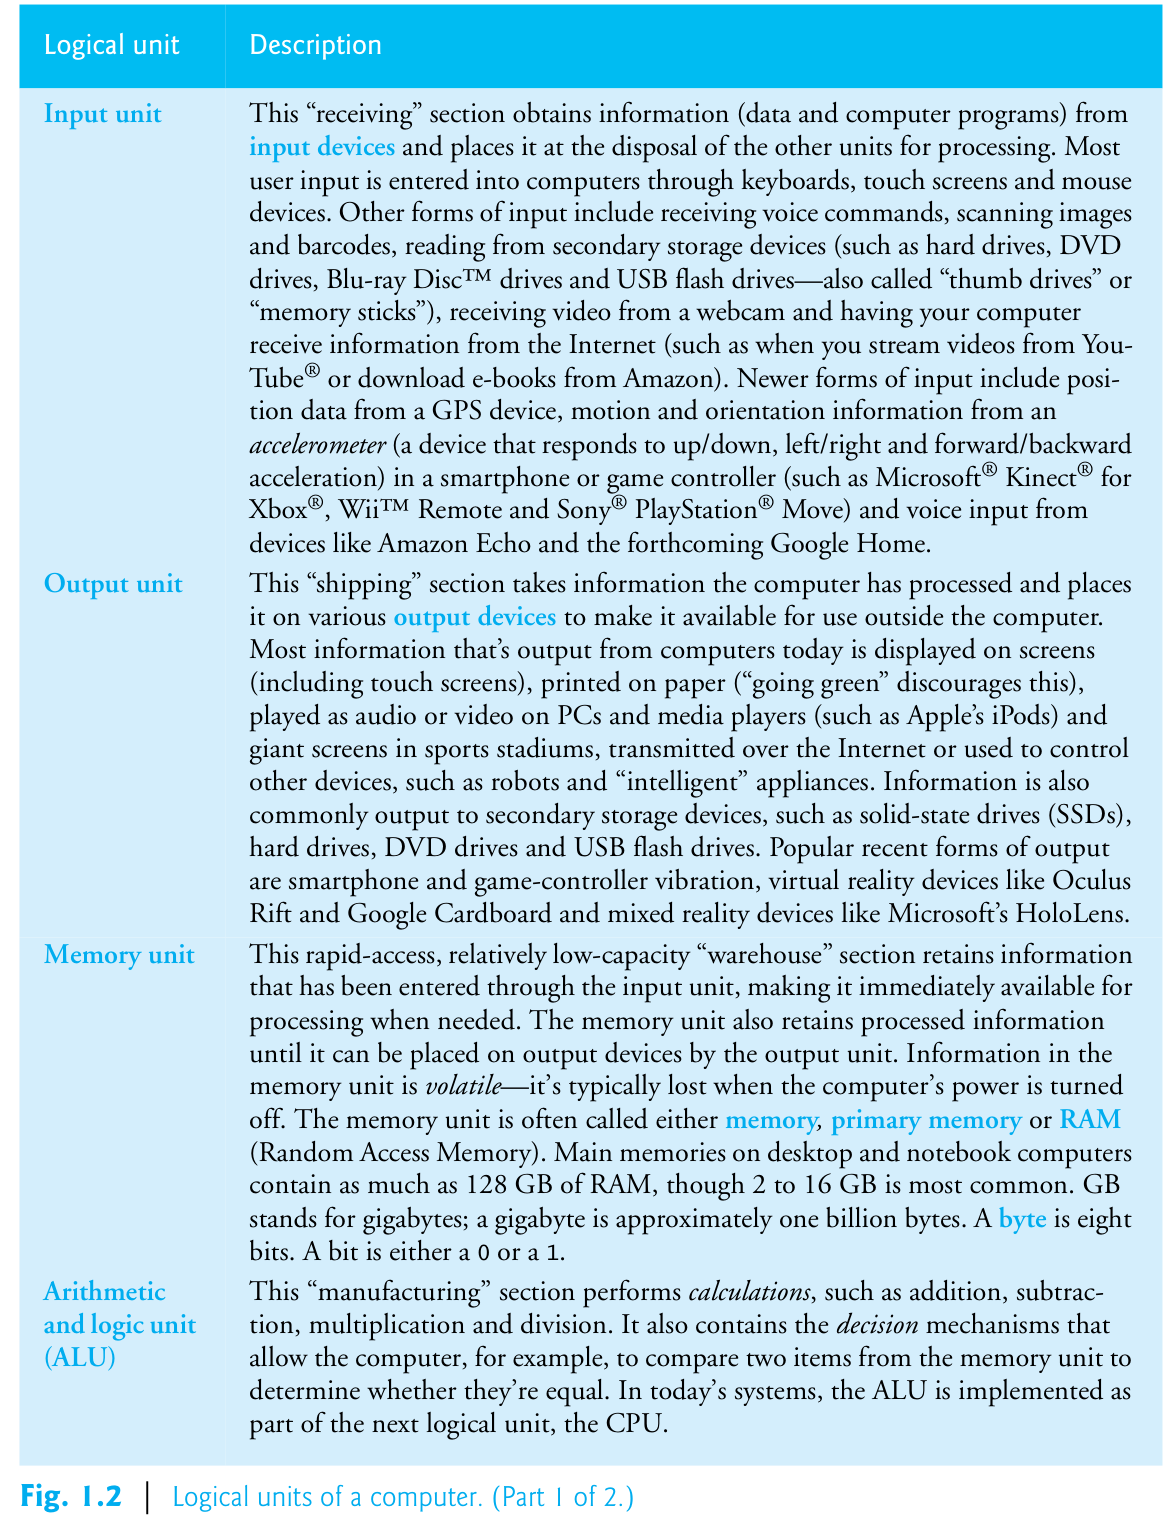
\includegraphics[width=\textwidth,height=0.78\textheight,keepaspectratio]{images/fig1_2_logical_units_p1.png}\\
      \scriptsize \color{gray} Hình 1.2: Các khối logic của máy tính (Phần 1/2 -- Deitel p.46)
    \end{column}
  \end{columns}
\end{frame}

% ==============================================================================
% SLIDE 10: 1.3.2 TỔ CHỨC MÁY TÍNH (PHẦN 2: ALU, CPU, STORAGE)
% ==============================================================================
\begin{frame}{1.3.2 Tổ chức Máy tính: 6 Khối Chức năng Logic (Phần 2)}
  \begin{columns}[c]
    \begin{column}{0.48\textwidth}
      \begin{block}{\textbf{3 Khối tiếp theo (Hình 1.2 Part 2):}}
        \begin{enumerate}
          \setcounter{enumi}{3}
          \item \textbf{Arithmetic and Logic Unit (ALU):}
          \begin{itemize}\scriptsize
            \item Bộ phận \textit{"nhà máy"} thực hiện tính toán số học (+, -, *, /) và so sánh logic ($=, <, >$).
          \end{itemize}
          \item \textbf{Central Processing Unit (CPU):}
          \begin{itemize}\scriptsize
            \item \textit{"Bộ não chỉ huy"} điều phối và giám sát toàn bộ hoạt động của tất cả các khối khác trong hệ thống.
            \item Hiện nay CPU tích hợp cả ALU và Control Unit trên cùng một chip silicon.
          \end{itemize}
          \item \textbf{Secondary Storage Unit (Bộ nhớ thứ cấp):}
          \begin{itemize}\scriptsize
            \item \textit{"Kho chứa hàng"} dài hạn, dung lượng lớn (SSD, HDD, USB).
            \item Dữ liệu \textbf{vẫn tồn tại khi tắt máy} (persistent / non-volatile).
          \end{itemize}
        \end{enumerate}
      \end{block}
    \end{column}
    \begin{column}{0.48\textwidth}
      \centering
      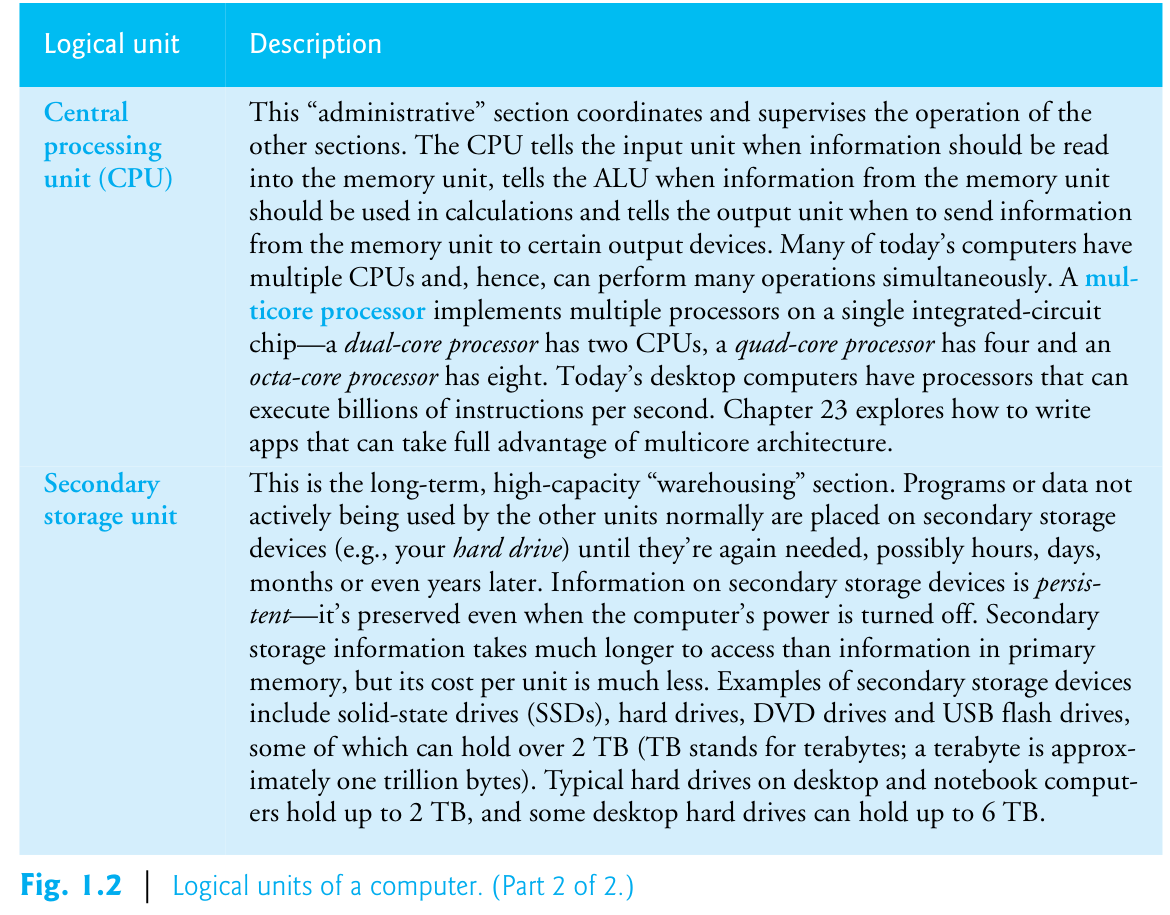
\includegraphics[width=\textwidth,height=0.78\textheight,keepaspectratio]{images/fig1_2_logical_units_p2.png}\\
      \scriptsize \color{gray} Hình 1.2: Các khối logic của máy tính (Phần 2/2 -- Deitel p.47)
    \end{column}
  \end{columns}
\end{frame}

% ==============================================================================
% SLIDE 11: SƠ ĐỒ LUỒNG DỮ LIỆU GIỮA CÁC KHỐI PHẦN CỨNG
% ==============================================================================
\begin{frame}{Sơ đồ Luồng Dữ liệu giữa 6 Khối Kiến trúc Máy tính}
  \centering
  \begin{tikzpicture}[scale=0.75, every node/.style={transform shape}]
    % Styles
    \tikzstyle{block} = [rectangle, draw=UniNavy, fill=UniLightBlue!60, text width=2.3cm, text centered, rounded corners, minimum height=1.1cm, font=\small\bfseries]
    \tikzstyle{cpu_block} = [rectangle, draw=CSharpPurple, fill=CSharpPurple!10, text width=2.3cm, text centered, rounded corners, minimum height=1.1cm, font=\small\bfseries]
    \tikzstyle{line} = [draw=UniNavy, -latex', line width=1.4pt]
    \tikzstyle{dline} = [draw=CSharpPurple, latex'-latex', line width=1.4pt]

    % Nodes
    \node [block] (input) {Input Unit\\(Bàn phím, Chuột)};
    \node [block, right=1.2cm of input] (memory) {Memory Unit\\(RAM Tạm thời)};
    \node [block, right=1.2cm of memory] (output) {Output Unit\\(Màn hình, Loa)};
    \node [block, below=1.0cm of memory] (storage) {Secondary Storage\\(SSD, HDD, USB)};
    \node [cpu_block, above=1.0cm of memory] (alu) {ALU\\(Tính toán \& So sánh)};
    \node [cpu_block, right=0.6cm of alu] (cu) {Control Unit\\(Điều khiển \& Lệnh)};

    % Container CPU
    \begin{scope}[on background layer]
      \node [draw=CSharpPurple, line width=1.3pt, fill=CSharpPurple!5, rounded corners, fit=(alu) (cu), inner sep=0.2cm, label=above:\textbf{\color{CSharpPurple}\footnotesize Central Processing Unit (CPU)}] (cpu_box) {};
    \end{scope}

    % Arrows
    \path [line] (input) -- node[above, font=\scriptsize] {Dữ liệu vào} (memory);
    \path [line] (memory) -- node[above, font=\scriptsize] {Kết quả xuất} (output);
    \path [dline] (memory) -- node[right, font=\scriptsize] {Load / Save} (storage);
    \path [dline] (memory) -- node[right, font=\scriptsize] {Fetch / Store} (alu);
    \path [draw=CSharpPurple, line width=1.2pt, -latex'] (cu) |- node[right, near start, font=\scriptsize] {Tín hiệu điều khiển} (memory);
  \end{tikzpicture}
  \vspace{-1mm}
  \begin{alertblock}{\textbf{Nguyên lý Vàng:}}
    \scriptsize Mọi dữ liệu muốn CPU xử lý \textbf{bắt buộc phải được nạp từ Secondary Storage vào RAM}. CPU không làm việc trực tiếp với ổ cứng SSD/HDD vì chênh lệch tốc độ hàng nghìn lần!
  \end{alertblock}
\end{frame}

% ==============================================================================
% SLIDE 12: 1.4 PHÂN CẤP DỮ LIỆU
% ==============================================================================
\begin{frame}{1.4 Phân cấp Dữ liệu (Data Hierarchy): Từ Bit đến Big Data}
  \begin{columns}[T]
    \begin{column}{0.48\textwidth}
      \begin{block}{\textbf{Các cấp độ dữ liệu (Thấp $\to$ Cao):}}
        \begin{itemize}\scriptsize
          \item \textbf{Bit (Binary Digit):} Đơn vị nhỏ nhất, mang giá trị \texttt{0} hoặc \texttt{1}.
          \item \textbf{Byte / Character:} Tập hợp 8 bits; biểu diễn 1 ký tự (mã ASCII, Unicode).
          \item \textbf{Field (Trường dữ liệu):} Nhóm các ký tự mang ý nghĩa (ví dụ: \texttt{Ten: "Judy"}).
          \item \textbf{Record (Bản ghi):} Nhóm các trường liên quan của 1 đối tượng (Mã SV, Họ tên, Điểm).
          \item \textbf{File (Tệp):} Tập hợp các bản ghi có cùng cấu trúc.
          \item \textbf{Database (Cơ sở dữ liệu):} Tập hợp nhiều tệp/bảng liên kết chặt chẽ.
          \item \textbf{Big Data:} Dữ liệu siêu lớn, tốc độ cao và đa dạng (Petabytes).
        \end{itemize}
      \end{block}
    \end{column}
    \begin{column}{0.48\textwidth}
      \centering
      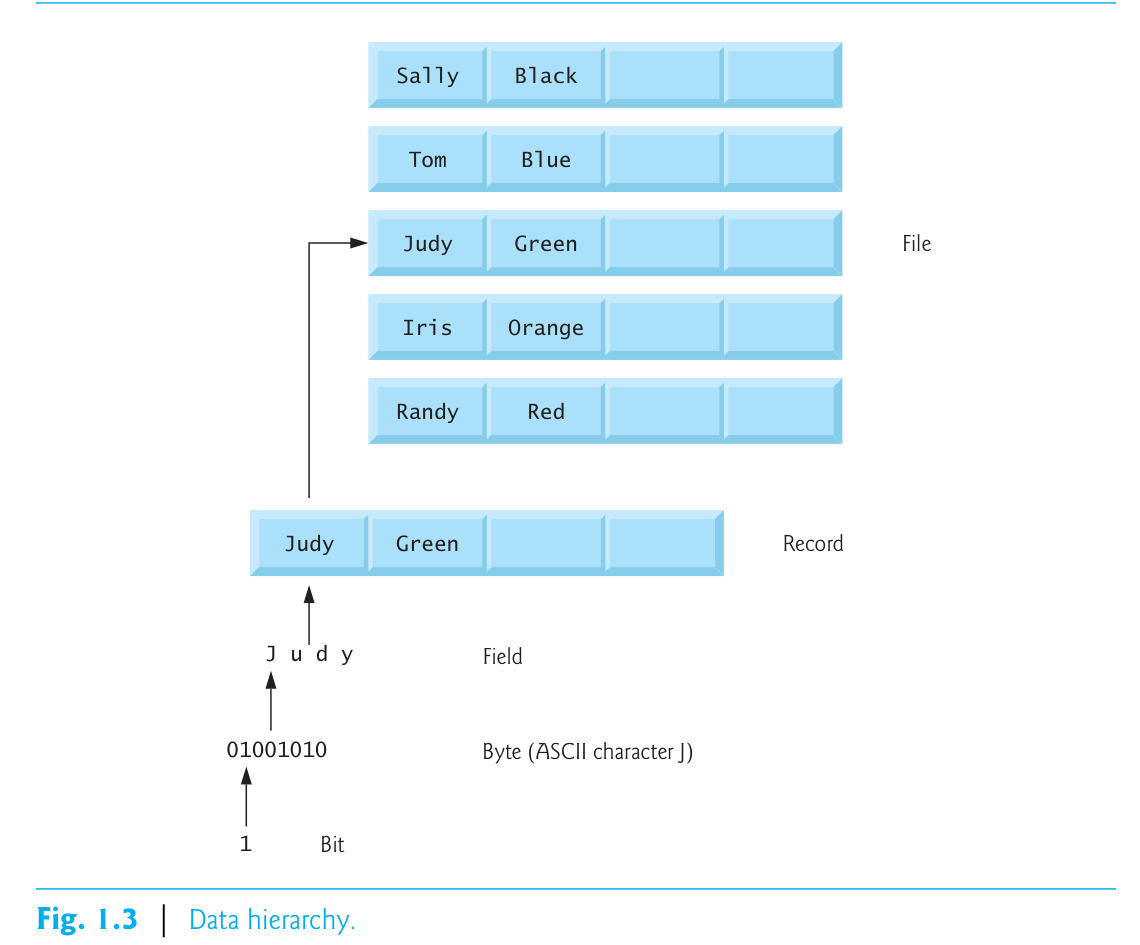
\includegraphics[width=\textwidth,height=0.68\textheight,keepaspectratio]{images/fig1_3_data_hierarchy.png}\\
      \scriptsize \color{gray} Hình 1.3: Mô hình phân cấp dữ liệu từ Bit đến File (Deitel p.48)
    \end{column}
  \end{columns}
\end{frame}

% ==============================================================================
% SLIDE 13: BẢNG ĐO LƯỜNG DUNG LƯỢNG BYTE
% ==============================================================================
\begin{frame}{Bảng Đo lường Dung lượng Dữ liệu: Từ KB đến YB}
  \begin{columns}[c]
    \begin{column}{0.48\textwidth}
      \begin{block}{\textbf{Quy ước tính toán trong Tin học:}}
        \begin{itemize}
          \item Vì máy tính dùng hệ nhị phân (cơ số 2), nên các bội số được định nghĩa theo lũy thừa $2^{10} = 1024$:
          \item $1\text{ KB} = 1024\text{ Bytes} \approx 10^3\text{ Bytes}$
          \item $1\text{ MB} = 1024\text{ KB} \approx 10^6\text{ Bytes}$
          \item $1\text{ GB} = 1024\text{ MB} \approx 10^9\text{ Bytes}$
          \item $1\text{ TB} = 1024\text{ GB} \approx 10^{12}\text{ Bytes}$
        \end{itemize}
      \end{block}
      \begin{alertblock}{\textbf{Lưu ý thực tế:}}
        Các nhà sản xuất ổ cứng thường tính $1\text{ GB} = 10^9$ bytes, do đó ổ cứng 500 GB hiển thị trong Windows chỉ khoảng 465 GB!
      \end{alertblock}
    \end{column}
    \begin{column}{0.48\textwidth}
      \centering
      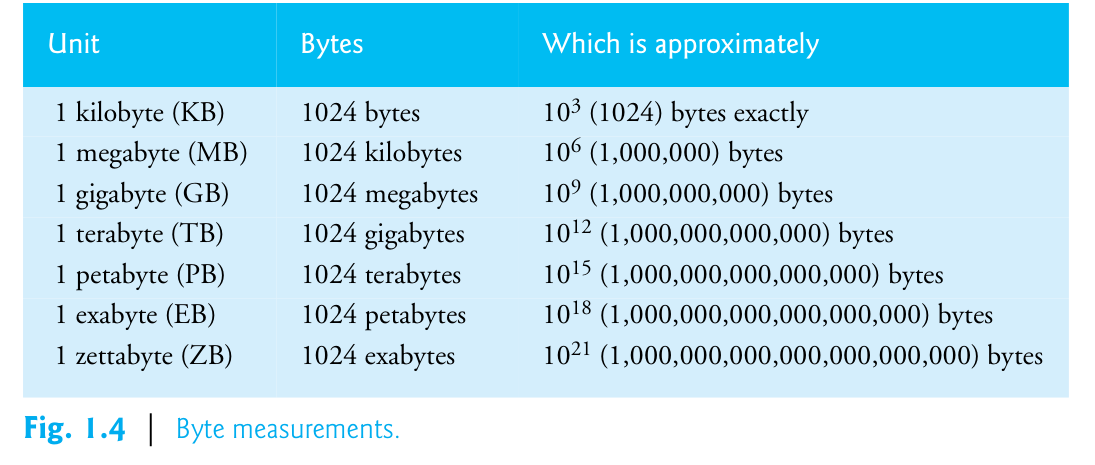
\includegraphics[width=\textwidth,height=0.75\textheight,keepaspectratio]{images/fig1_4_byte_measurements.png}\\
      \scriptsize \color{gray} Hình 1.4: Bảng các đơn vị đo lường Byte (Deitel p.50)
    \end{column}
  \end{columns}
\end{frame}

% ==============================================================================
% SLIDE 14: [CHECKPOINT 1] TRẮC NGHIỆM TIẾT 1
% ==============================================================================
\begin{frame}{[CHECKPOINT 1] Kiểm tra Nhanh Kiến thức Tiết 1}
  \begin{tcolorbox}[colback=UniOrange!5,colframe=UniOrange,top=1.5mm,bottom=1.5mm,title=\textbf{Câu hỏi 1: Khối chức năng nào thực hiện phép so sánh logic (A > B)?}]
    \begin{itemize}\scriptsize
      \item[A.] Input unit
      \item[B.] Memory unit (RAM)
      \item[C.] \textbf{Arithmetic and Logic Unit (ALU)} \hfill \textit{\color{UniGreen}\textbf{[ĐÁP ÁN ĐÚNG]}}
      \item[D.] Secondary storage unit
    \end{itemize}
  \end{tcolorbox}
  \vskip 1mm
  \begin{tcolorbox}[colback=UniNavy!5,colframe=UniNavy,top=1.5mm,bottom=1.5mm,title=\textbf{Câu hỏi 2: Cấp độ nào trong phân cấp dữ liệu bao gồm nhiều trường (fields) có liên quan?}]
    \begin{itemize}\scriptsize
      \item[A.] Byte
      \item[B.] \textbf{Record (Bản ghi)} \hfill \textit{\color{UniGreen}\textbf{[ĐÁP ÁN ĐÚNG]}}
      \item[C.] Bit
      \item[D.] Character
    \end{itemize}
  \end{tcolorbox}
\end{frame}

% ==============================================================================
% SLIDE 15: [HANDS-ON LAB 1] THỰC HÀNH KHẢO SÁT HỆ THỐNG
% ==============================================================================
\begin{frame}[fragile]{[HANDS-ON LAB 1] Khảo sát Phần cứng \& Tính toán Nhị phân}
  \begin{exampleblock}{\textbf{Nhiệm vụ Thực hành (15 Phút tại phòng máy IT26M):}}
    \begin{enumerate}
      \item Mở \textbf{Task Manager} (Ctrl + Shift + Esc) $\to$ chọn tab \textbf{Performance}:
      \begin{itemize}
        \item Ghi lại: Tên CPU, Xung nhịp cơ bản (GHz), Số nhân (Cores), Số luồng (Logical Processors).
        \item Kiểm tra dung lượng RAM và tốc độ (Speed MHz).
      \end{itemize}
      \item Mở \textbf{Command Prompt} (CMD) và gõ lệnh xem thông số vi xử lý:
    \end{enumerate}
  \end{exampleblock}
\begin{lstlisting}[style=terminalStyle]
C:\> wmic cpu get name, numberofcores, numberoflogicalprocessors, maxclockspeed
Name                                              MaxClockSpeed  NumberOfCores  NumberOfLogicalProcessors
Intel(R) Core(TM) i7-13700H CPU @ 2.40GHz        2400           14             20
\end{lstlisting}
  \begin{block}{\textbf{Bài tập nhị phân tại chỗ:}}
    Chuyển đổi số nguyên $45_{10}$ sang nhị phân $\to$ Đáp án: $101101_2$ (gồm 6 bits).
  \end{block}
\end{frame}

% ==============================================================================
% SLIDE 16: TỔNG KẾT TIẾT 1
% ==============================================================================
\begin{frame}{Tổng kết Trọng tâm Tiết 1}
  \begin{columns}[T]
    \begin{column}{0.48\textwidth}
      \begin{tcolorbox}[colback=UniLightBlue,colframe=UniNavy,title=\textbf{3 Khái niệm Cốt lõi Tiết 1}]
        \begin{enumerate}
          \item \textbf{Định luật Moore:} Động lực giúp phần cứng tăng gấp đôi hiệu năng sau mỗi 18-24 tháng.
          \item \textbf{6 Khối logic:} Input, Output, Memory, ALU, CPU, Secondary Storage.
          \item \textbf{Phân cấp dữ liệu:} Bit $\to$ Byte $\to$ Field $\to$ Record $\to$ File $\to$ Database.
        \end{enumerate}
      \end{tcolorbox}
    \end{column}
    \begin{column}{0.48\textwidth}
      \begin{tcolorbox}[colback=CSharpPurple!10,colframe=CSharpPurple,title=\textbf{Chuẩn bị bước sang Tiết 2}]
        \begin{itemize}
          \item Làm thế nào để ra lệnh cho phần cứng máy tính làm việc theo ý muốn?
          \item Các ngôn ngữ lập trình đã tiến hóa như thế nào?
          \item Tại sao Microsoft lại phát minh ra C\# và nền tảng .NET?
        \end{itemize}
        \vskip 2mm
        \centering \textbf{\color{UniOrange} Giải lao 5 phút trước khi vào Tiết 2!}
      \end{tcolorbox}
    \end{column}
  \end{columns}
\end{frame}

% ==============================================================================
% SLIDE 17: TIẾT 2 TITLE
% ==============================================================================
\begin{frame}
  \vfill
  \centering
  \begin{beamercolorbox}[sep=8pt,center,shadow=true,rounded=true]{palette secondary}
    \usebeamerfont{title}\Huge \textbf{TIẾT 2: TIẾN HÓA NGÔN NGỮ,}\\[2mm]
    \Large \textbf{CÔNG NGHỆ ĐỐI TƯỢNG \& KIẾN TRÚC .NET}
  \end{beamercolorbox}
  \vfill
\end{frame}

% ==============================================================================
% SLIDE 18: 1.5 CÁC THẾ HỆ NGÔN NGỮ LẬP TRÌNH
% ==============================================================================
\begin{frame}{1.5 Các Thế hệ Ngôn ngữ Lập trình (Language Evolution)}
  \begin{columns}[T]
    \begin{column}{0.48\textwidth}
      \begin{block}{\textbf{1. Ngôn ngữ máy (Machine Language)}}
        \begin{itemize}
          \item Là ngôn ngữ \textbf{duy nhất} phần cứng CPU có thể hiểu và thực thi trực tiếp.
          \item Cấu thành từ các chuỗi số nhị phân \texttt{0} và \texttt{1}.
          \item Phụ thuộc chặt chẽ vào kiến trúc phần cứng máy tính (Machine-dependent).
          \item Cực kỳ khó viết, dễ sai sót và không thể bảo trì bởi con người.
        \end{itemize}
      \end{block}
    \end{column}
    \begin{column}{0.48\textwidth}
      \begin{block}{\textbf{2. Hợp ngữ (Assembly Language)}}
        \begin{itemize}
          \item Sử dụng các từ gợi nhớ tiếng Anh (Mnemonics) viết tắt: \texttt{LOAD}, \texttt{ADD}, \texttt{STORE}.
          \item Cần chương trình \textbf{Assembler} để dịch hợp ngữ sang ngôn ngữ máy.
          \item Vẫn phụ thuộc vào dòng vi xử lý cụ thể, tốc độ viết code vẫn rất chậm.
        \end{itemize}
      \end{block}
    \end{column}
  \end{columns}
  \vskip 2mm
  \begin{exampleblock}{\textbf{3. Ngôn ngữ bậc cao (High-Level Language): C, C++, Java, C\#, Python}}
    Cú pháp gần với ngôn ngữ tự nhiên tiếng Anh và ký hiệu toán học; độc lập với phần cứng.
  \end{exampleblock}
\end{frame}

% ==============================================================================
% SLIDE 19: BIÊN DỊCH VS THÔNG DỊCH
% ==============================================================================
\begin{frame}{Biên dịch (Compiler) vs Thông dịch (Interpreter)}
  \begin{columns}[T]
    \begin{column}{0.48\textwidth}
      \begin{block}{\textbf{Trình biên dịch (Compiler)}}
        \begin{itemize}
          \item Dịch \textbf{toàn bộ} mã nguồn bậc cao thành tệp mã máy (Machine code) trước khi thực thi.
          \item Quá trình biên dịch tốn thời gian ban đầu nhưng chương trình chạy \textbf{cực kỳ nhanh}.
          \item Báo lỗi cú pháp toàn diện trước khi cho phép chạy chương trình.
          \item \textit{Đại diện:} C, C++, Rust, Go.
        \end{itemize}
      \end{block}
    \end{column}
    \begin{column}{0.48\textwidth}
      \begin{block}{\textbf{Trình thông dịch (Interpreter)}}
        \begin{itemize}
          \item Đọc và dịch \textbf{từng dòng lệnh một}, chạy trực tiếp lệnh đó rồi mới sang dòng kế tiếp.
          \item Chạy ngay không cần chờ biên dịch, nhưng tốc độ thực thi \textbf{chậm hơn đáng kể}.
          \item Lỗi ở dòng nào chỉ phát hiện khi máy tính chạy đến dòng đó.
          \item \textit{Đại diện:} Python, JavaScript, Ruby, PHP.
        \end{itemize}
      \end{block}
    \end{column}
  \end{columns}
  \vskip 2mm
  \begin{alertblock}{\textbf{Cơ chế Lai (Hybrid Approach) trong C\# / Java:}}
    Biên dịch mã nguồn thành \textbf{Mã trung gian (MSIL / Bytecode)}, sau đó dùng \textbf{JIT Compiler} trong máy ảo để dịch sang mã máy siêu tốc khi ứng dụng khởi chạy!
  \end{alertblock}
\end{frame}

% ==============================================================================
% SLIDE 20: 1.6 CÔNG NGHỆ ĐỐI TƯỢNG (OBJECT TECHNOLOGY)
% ==============================================================================
\begin{frame}{1.6 Công nghệ Đối tượng (Object Technology)}
  \begin{columns}[c]
    \begin{column}{0.55\textwidth}
      \begin{block}{\textbf{Tư duy Hướng đối tượng trong Lập trình:}}
        \begin{itemize}
          \item Trong thế giới thực, mọi vật xung quanh chúng ta đều là các \textbf{Đối tượng (Objects)}: ô tô, điện thoại, con người, tài khoản.
          \item Mỗi đối tượng đều có hai thành phần:
          \begin{enumerate}
            \item \textbf{Thuộc tính (Attributes / Properties):} Màu sắc, kích thước, số dư tài khoản.
            \item \textbf{Hành vi (Behaviors / Methods):} Chạy, dừng, tăng tốc, rút tiền, chuyển khoản.
          \end{enumerate}
        \end{itemize}
      \end{block}
    \end{column}
    \begin{column}{0.42\textwidth}
      \begin{tcolorbox}[colback=CSharpPurple!10,colframe=CSharpPurple,title=\textbf{Mục tiêu Tối thượng của OOP}]
        \centering
        \textbf{\large Tái sử dụng Phần mềm\\(Software Reuse)}
        \vskip 2mm
        \scriptsize Thay vì tự gõ lại mọi dòng code từ đầu, ta sử dụng các lớp đối tượng có sẵn đạt chuẩn chất lượng cao, giúp tăng năng suất gấp nhiều lần.
      \end{tcolorbox}
    \end{column}
  \end{columns}
\end{frame}

% ==============================================================================
% SLIDE 21: CLASS VS OBJECT: MÔ HÌNH Ô TÔ THỰC TẾ
% ==============================================================================
\begin{frame}{Phân biệt Lớp (Class) và Đối tượng (Object)}
  \begin{columns}[c]
    \begin{column}{0.48\textwidth}
      \begin{tcolorbox}[colback=UniNavy!5,colframe=UniNavy,title=\textbf{Lớp (Class) = Bản vẽ thiết kế}]
        \begin{itemize}
          \item Là khuôn mẫu (Blueprint / Template) định nghĩa cấu trúc dữ liệu và hành vi chung.
          \item \textit{Ví dụ:} Bản vẽ thiết kế kỹ thuật ô tô trên giấy: chỉ định xe có 4 bánh, vô lăng, màu sơn, động cơ.
          \item Bản vẽ \textbf{không thể tự nổ máy hay chạy trên đường}!
        \end{itemize}
      \end{tcolorbox}
    \end{column}
    \begin{column}{0.48\textwidth}
      \begin{tcolorbox}[colback=UniGreen!5,colframe=UniGreen,title=\textbf{Đối tượng (Object) = Thực thể cụ thể}]
        \begin{itemize}
          \item Là một thể hiện cụ thể (Instance) được chế tạo từ bản vẽ lớp.
          \item \textit{Ví dụ:} Chiếc xe VinFast màu đỏ biển số \texttt{43A-12345} thực sự lăn bánh ngoài đời.
          \item Từ 1 Class có thể tạo ra \textbf{vô số Objects} với các giá trị thuộc tính riêng biệt!
        \end{itemize}
      \end{tcolorbox}
    \end{column}
  \end{columns}
  \vskip 2mm
  \begin{exampleblock}{\textbf{Cú pháp khởi tạo trong C\#:}}
    \texttt{Car myCar = new Car("VinFast VF8", "Do"); // Toán tử new sinh đối tượng trong RAM}
  \end{exampleblock}
\end{frame}

% ==============================================================================
% SLIDE 22: CÁC TRỤ CỘT OOP (ENCAPSULATION, INHERITANCE)
% ==============================================================================
\begin{frame}{Các Trụ cột Công nghệ Đối tượng trong C\#}
  \begin{columns}[T]
    \begin{column}{0.48\textwidth}
      \begin{block}{\textbf{1. Đóng gói (Encapsulation)}}
        \begin{itemize}
          \item Gom nhóm dữ liệu và phương thức xử lý vào trong một đơn vị Class duy nhất.
          \item \textbf{Che giấu thông tin (Information Hiding):} Người lái xe chỉ cần đạp chân ga để tăng tốc, không cần biết chi tiết quá trình bơm nhiên liệu vào buồng đốt!
          \item Bảo vệ dữ liệu nội bộ không bị can thiệp trái phép từ bên ngoài.
        \end{itemize}
      \end{block}
    \end{column}
    \begin{column}{0.48\textwidth}
      \begin{block}{\textbf{2. Kế thừa (Inheritance)}}
        \begin{itemize}
          \item Cho phép tạo ra một Class mới dựa trên một Class đã có sẵn.
          \item Lớp con thừa hưởng toàn bộ thuộc tính và hành vi của lớp cha, đồng thời có thể bổ sung tính năng riêng.
          \item \textit{Ví dụ:} \texttt{XeDien} kế thừa từ \texttt{OTo}, bổ sung thêm thuộc tính \texttt{DungLuongPin}.
        \end{itemize}
      \end{block}
    \end{column}
  \end{columns}
  \vskip 2mm
  \begin{block}{\textbf{3. Đa hình (Polymorphism):}}
    Cho phép các đối tượng thuộc các lớp khác nhau phản ứng với cùng một thông điệp theo những cách riêng biệt (sẽ học sâu ở Chương 8 \& 9).
  \end{block}
\end{frame}

% ==============================================================================
% SLIDE 23: 1.7 INTERNET VÀ WORLD WIDE WEB
% ==============================================================================
\begin{frame}{1.7 Internet và World Wide Web}
  \begin{block}{\textbf{Các cột mốc tiến hóa mạng thông tin toàn cầu:}}
    \begin{itemize}
      \item \textbf{ARPANET (1969):} Tiền thân của Internet, do Bộ Quốc phòng Mỹ tài trợ, tiên phong kỹ thuật chuyển mạch gói (Packet Switching).
      \item \textbf{Giao thức TCP/IP:} Bộ giao thức mạng nền tảng kết nối các mạng máy tính khác biệt trên thế giới.
      \item \textbf{World Wide Web (1989):} Tim Berners-Lee phát minh siêu văn bản (HTML) và giao thức HTTP, biến Internet thành không gian chia sẻ tài liệu toàn cầu.
      \item \textbf{Web 2.0 (Thập niên 2000):} Chuyển từ web đọc tĩnh sang web tương tác người dùng (Facebook, YouTube, Wikipedia, Cloud SaaS).
      \item \textbf{Điện toán đám mây (Cloud Computing - Microsoft Azure):} Thuê năng lực tính toán và lưu trữ quy mô toàn cầu theo nhu cầu thực tế.
      \item \textbf{Internet of Things (IoT):} Hàng tỷ thiết bị thông minh (đồng hồ, TV, cảm biến xe) kết nối và trao đổi dữ liệu qua Internet.
    \end{itemize}
  \end{block}
\end{frame}

% ==============================================================================
% SLIDE 24: 1.8 NGÔN NGỮ C# VÀ ĐẶC TRƯNG VƯỢT TRỘI
% ==============================================================================
\begin{frame}{1.8 Ngôn ngữ C\#: Lịch sử Hình thành \& Chuẩn hóa}
  \begin{columns}[c]
    \begin{column}{0.55\textwidth}
      \begin{block}{\textbf{Lịch sử ra đời:}}
        \begin{itemize}
          \item Được Microsoft công bố vào năm 2000, đi cùng sáng kiến .NET.
          \item Người đứng đầu nhóm thiết kế: \textbf{Anders Hejlsberg} (Kỹ sư trưởng huyền thoại).
          \item C\# được chuẩn hóa quốc tế bởi \textbf{ECMA (ECMA-334)} và \textbf{ISO/IEC (ISO/IEC 23270)}.
        \end{itemize}
      \end{block}
      \begin{exampleblock}{\textbf{Nguồn gốc tên gọi C\#:}}
        Dấu thăng (\#) mượn từ âm nhạc (thăng tiến), đồng thời ghép từ 4 dấu cộng ($++$ của C++ xếp chồng lên nhau thành $\#$), biểu thị sự kế thừa và nâng cấp toàn diện!
      \end{exampleblock}
    \end{column}
    \begin{column}{0.42\textwidth}
      \begin{tcolorbox}[colback=CSharpPurple!10,colframe=CSharpPurple,title=\textbf{Đặc trưng Cốt lõi của C\#}]
        \begin{itemize}\scriptsize
          \item Hướng đối tượng 100\% (Pure OOP)
          \item Định kiểu mạnh mẽ \& An toàn (Type-safe)
          \item Thu gom rác tự động (Garbage Collection)
          \item Hỗ trợ lập trình trực quan (Visual)
          \item Hỗ trợ xử lý bất đồng bộ (\texttt{async/await})
          \item Đa nền tảng (Cross-platform)
        \end{itemize}
      \end{tcolorbox}
    \end{column}
  \end{columns}
\end{frame}

% ==============================================================================
% SLIDE 25: CÁC PHONG CÁCH LẬP TRÌNH TRONG C#
% ==============================================================================
\begin{frame}{Các Phong cách Lập trình Đa dạng trong C\#}
  \begin{columns}[T]
    \begin{column}{0.48\textwidth}
      \begin{block}{\textbf{1. Lập trình Hướng sự kiện (Event-Driven)}}
        \begin{itemize}
          \item Ứng dụng phản hồi lại các sự kiện (Events) do người dùng kích hoạt: Click chuột, gõ phím, di chuột.
          \item Cốt lõi của các ứng dụng GUI hiện đại.
        \end{itemize}
      \end{block}
      \begin{block}{\textbf{2. Lập trình Trực quan (Visual Programming)}}
        \begin{itemize}
          \item Kéo - thả các điều khiển (Button, TextBox, Grid) trực tiếp trên Form Designer thay vì viết code giao diện thủ công.
        \end{itemize}
      \end{block}
    \end{column}
    \begin{column}{0.48\textwidth}
      \begin{block}{\textbf{3. Lập trình Tổng quát (Generic Programming)}}
        \begin{itemize}
          \item Viết thuật toán và cấu trúc dữ liệu tổng quát cho mọi kiểu dữ liệu mà vẫn đảm bảo Type-Safety (ví dụ \texttt{List<T>}).
        \end{itemize}
      \end{block}
      \begin{block}{\textbf{4. Lập trình Bất đồng bộ (Async / Await)}}
        \begin{itemize}
          \item Thực thi các tác vụ tốn thời gian (I/O, gọi API mạng, truy vấn CSDL) mà \textbf{không làm đơ / treo giao diện} người dùng.
        \end{itemize}
      \end{block}
    \end{column}
  \end{columns}
\end{frame}

% ==============================================================================
% SLIDE 26: 1.9 NỀN TẢNG MICROSOFT .NET
% ==============================================================================
\begin{frame}{1.9 Nền tảng Microsoft .NET: Tầm nhìn Kiến trúc}
  \begin{block}{\textbf{Sáng kiến Microsoft .NET (Ra mắt năm 2000):}}
    Một nền tảng phần mềm toàn diện cho phép phát triển, triển khai và thực thi ứng dụng dễ dàng trên Internet và mạng nội bộ.
  \end{block}
  \begin{columns}[T]
    \begin{column}{0.48\textwidth}
      \begin{tcolorbox}[colback=UniLightBlue,colframe=UniBlue,title=\textbf{1. Thư viện Lớp (.NET FCL)}]
        \begin{itemize}\scriptsize
          \item Hàng chục nghìn lớp có sẵn được tối ưu hóa hiệu năng cao.
          \item Cung cấp giải pháp cho: Thao tác tệp (File I/O), Mạng (Networking), CSDL (ADO.NET, Entity Framework), Bảo mật, Giao diện (WinForms, WPF).
          \item Tái sử dụng tối đa, tiết kiệm 70\% thời gian gõ code.
        \end{itemize}
      \end{tcolorbox}
    \end{column}
    \begin{column}{0.48\textwidth}
      \begin{tcolorbox}[colback=CSharpPurple!10,colframe=CSharpPurple,title=\textbf{2. Máy ảo CLR (Common Language Runtime)}]
        \begin{itemize}\scriptsize
          \item Trái tim vận hành của toàn bộ hệ sinh thái .NET.
          \item Quản lý toàn bộ vòng đời thực thi ứng dụng.
          \item Ẩn giấu phần cứng và hệ điều hành bên dưới đối với lập trình viên.
          \item Cung cấp các dịch vụ quản lý tự động: Cấp phát bộ nhớ, thu gom rác, kiểm tra bảo mật.
        \end{itemize}
      \end{tcolorbox}
    \end{column}
  \end{columns}
\end{frame}

% ==============================================================================
% SLIDE 27: MANAGED CODE & CÁC DỊCH VỤ CỦA CLR
% ==============================================================================
\begin{frame}{Khái niệm Managed Code (Mã được Quản lý)}
  \begin{columns}[T]
    \begin{column}{0.48\textwidth}
      \begin{block}{\textbf{Managed Code (Mã được quản lý)}}
        \begin{itemize}
          \item Là mã nguồn được biên dịch ra mã trung gian MSIL và \textbf{chạy dưới sự giám sát hoàn toàn của CLR}.
          \item C\#, VB.NET, F\# mặc định luôn là Managed Code.
          \item \textbf{Lợi ích to lớn:}
          \begin{itemize}
            \item Không lo rò rỉ bộ nhớ (Memory Leaks).
            \item Ngăn chặn lỗi ghi đè vùng nhớ (Buffer Overflow).
            \item Bắt lỗi ngoại lệ (Exceptions) an toàn giữa các ngôn ngữ khác nhau.
          \end{itemize}
        \end{itemize}
      \end{block}
    \end{column}
    \begin{column}{0.48\textwidth}
      \begin{block}{\textbf{Unmanaged Code (Mã không quản lý)}}
        \begin{itemize}
          \item Được biên dịch trực tiếp sang mã máy nhị phân của CPU (ví dụ C, C++ truyền thống).
          \item Không có máy ảo CLR quản lý.
          \item Lập trình viên phải tự quản lý từng byte bộ nhớ (\texttt{malloc}, \texttt{free}, con trỏ).
          \item Nếu có lỗi con trỏ có thể làm sập toàn bộ hệ điều hành (Crash / BSoD).
        \end{itemize}
      \end{block}
    \end{column}
  \end{columns}
\end{frame}

% ==============================================================================
% SLIDE 28: KIẾN TRÚC THỰC THI .NET (MSIL & JIT)
% ==============================================================================
\begin{frame}{Kiến trúc Thực thi .NET: Mã nguồn $\to$ MSIL $\to$ CLR JIT}
  \centering
  \begin{tikzpicture}[scale=0.78, every node/.style={transform shape}]
    % Nodes
    \node [rectangle, draw=CSharpPurple, fill=CSharpPurple!10, rounded corners, minimum width=2.2cm, minimum height=1cm, font=\small\bfseries, align=center] (src_cs) {Mã nguồn C\#\\(\texttt{*.cs})};
    \node [rectangle, draw=UniBlue, fill=UniBlue!10, rounded corners, minimum width=2.2cm, minimum height=1cm, right=0.6cm of src_cs, font=\small\bfseries, align=center] (compiler) {Trình biên dịch C\#\\(\texttt{csc.exe})};
    \node [rectangle, draw=UniNavy, fill=UniNavy!15, rounded corners, minimum width=2.6cm, minimum height=1cm, right=0.6cm of compiler, font=\small\bfseries, align=center] (msil) {Mã trung gian MSIL\\+ Metadata (\texttt{*.dll})};
    \node [rectangle, draw=UniOrange, fill=UniOrange!15, rounded corners, minimum width=2.2cm, minimum height=1cm, right=0.6cm of msil, font=\small\bfseries, align=center] (jit) {CLR JIT Compiler\\(Dịch thời gian thực)};
    \node [rectangle, draw=UniGreen, fill=UniGreen!20, rounded corners, minimum width=2.2cm, minimum height=1cm, right=0.6cm of jit, font=\small\bfseries, align=center] (native) {Mã máy bản địa\\(Native Code)};

    % Hardware
    \node [rectangle, draw=UniDark, fill=UniDark, text=white, rounded corners, minimum width=2.2cm, minimum height=0.7cm, below=0.5cm of native, font=\small\bfseries, align=center] (cpu) {CPU / Phần cứng};

    % Arrows
    \draw [draw=CSharpPurple, -latex', line width=1.4pt] (src_cs) -- (compiler);
    \draw [draw=UniBlue, -latex', line width=1.4pt] (compiler) -- (msil);
    \draw [draw=UniNavy, -latex', line width=1.4pt] (msil) -- (jit);
    \draw [draw=UniOrange, -latex', line width=1.4pt] (jit) -- (native);
    \draw [draw=UniGreen, -latex', line width=1.4pt] (native) -- (cpu);

    % Groups
    \begin{scope}[on background layer]
      \node [draw=black!30, dashed, fill=black!2, rounded corners, fit=(src_cs) (compiler), inner sep=0.15cm, label=above:\textbf{\footnotesize Giai đoạn Biên dịch (Compile Time)}] {};
      \node [draw=CSharpPurple, line width=1.2pt, fill=CSharpPurple!5, rounded corners, fit=(jit) (native) (cpu), inner sep=0.2cm, label=below:\textbf{\color{CSharpPurple}\footnotesize Môi trường Máy ảo CLR (Runtime Execution)}] {};
    \end{scope}
  \end{tikzpicture}
  \vspace{-1mm}
  \begin{alertblock}{\textbf{Vai trò của MSIL (Microsoft Intermediate Language):}}
    \scriptsize MSIL không phải mã máy của Intel hay ARM. Nhờ đó, tệp \texttt{*.dll} có thể mang sang bất kỳ máy tính nào chạy Windows, Linux hay macOS có cài đặt CLR để thực thi mượt mà!
  \end{alertblock}
\end{frame}

% ==============================================================================
% SLIDE 29: ĐỘC LẬP NỀN TẢNG & .NET CORE / .NET 8
% ==============================================================================
\begin{frame}{1.9.3 Độc lập Nền tảng (Platform Independence)}
  \begin{columns}[c]
    \begin{column}{0.55\textwidth}
      \begin{block}{\textbf{Triết lý "Write Once, Run Anywhere":}}
        \begin{itemize}
          \item Lập trình viên chỉ cần viết và biên dịch code một lần thành MSIL.
          \item Bất kỳ hệ điều hành nào có máy ảo CLR tương thích đều có thể thực thi chương trình mà \textbf{không cần sửa hay biên dịch lại mã nguồn}.
          \item Tiết kiệm hàng triệu USD chi phí chuyển đổi (porting) phần mềm cho doanh nghiệp.
        \end{itemize}
      \end{block}
    \end{column}
    \begin{column}{0.42\textwidth}
      \begin{tcolorbox}[colback=UniLightBlue,colframe=UniBlue,title=\textbf{Sự tiến hóa của .NET}]
        \begin{itemize}\scriptsize
          \item \textbf{.NET Framework (2002 - 2019):} Ban đầu chủ yếu tối ưu hóa cho hệ điều hành Windows.
          \item \textbf{.NET Core (2016):} Viết lại hoàn toàn với mã nguồn mở, hoạt động siêu tốc trên Windows, Linux, macOS.
          \item \textbf{.NET 5 $\to$ 8 $\to$ 9 (Hiện đại):} Hợp nhất toàn bộ hệ sinh thái .NET thành một nền tảng duy nhất đẳng cấp thế giới.
        \end{itemize}
      \end{tcolorbox}
    \end{column}
  \end{columns}
\end{frame}

% ==============================================================================
% SLIDE 30: TƯƠNG TÁC ĐA NGÔN NGỮ (LANGUAGE INTEROPERABILITY)
% ==============================================================================
\begin{frame}{1.9.4 Khả năng Tương tác Đa ngôn ngữ (Language Interoperability)}
  \begin{columns}[c]
    \begin{column}{0.48\textwidth}
      \begin{block}{\textbf{Tự do lựa chọn Ngôn ngữ:}}
        \begin{itemize}
          \item Nền tảng .NET không bắt buộc lập trình viên phải dùng chung một ngôn ngữ.
          \item Lập trình viên có thể viết Module A bằng \textbf{C\#}, Module B bằng \textbf{Visual Basic}, và Module C bằng \textbf{F\#}.
          \item Tất cả đều được biên dịch về cùng một chuẩn \textbf{mã trung gian MSIL}!
        \end{itemize}
      \end{block}
    \end{column}
    \begin{column}{0.48\textwidth}
      \begin{exampleblock}{\textbf{Sức mạnh Tích hợp Không biên giới:}}
        \begin{itemize}
          \item Một lớp viết bằng C\# có thể \textbf{kế thừa trực tiếp} một lớp viết bằng Visual Basic.
          \item Một phương thức viết bằng C\# có thể bắt ngoại lệ (Exception) do mã F\# ném ra.
          \item Toàn bộ thư viện .NET Framework Class Library (FCL) được chia sẻ bình đẳng cho tất cả các ngôn ngữ .NET.
        \end{itemize}
      \end{exampleblock}
    \end{column}
  \end{columns}
\end{frame}

% ==============================================================================
% SLIDE 31: [CHECKPOINT 2] TRẮC NGHIỆM TIẾT 2
% ==============================================================================
\begin{frame}{[CHECKPOINT 2] Kiểm tra Nhanh Kiến thức Tiết 2}
  \begin{tcolorbox}[colback=UniOrange!5,colframe=UniOrange,top=1.5mm,bottom=1.5mm,title=\textbf{Câu hỏi 1: Mã nguồn C\# khi biên dịch lần đầu sẽ tạo ra loại mã nào?}]
    \begin{itemize}\scriptsize
      \item[A.] Mã máy nhị phân của CPU Intel x86/x64
      \item[B.] \textbf{Mã trung gian Microsoft Intermediate Language (MSIL / CIL)} \hfill \textit{\color{UniGreen}\textbf{[ĐÁP ÁN ĐÚNG]}}
      \item[C.] Mã hợp ngữ Assembly
      \item[D.] Mã thông dịch Python bytecode
    \end{itemize}
  \end{tcolorbox}
  \vskip 1mm
  \begin{tcolorbox}[colback=CSharpPurple!5,colframe=CSharpPurple,top=1.5mm,bottom=1.5mm,title=\textbf{Câu hỏi 2: Thành phần nào trong CLR dịch MSIL sang mã máy khi ứng dụng chạy?}]
    \begin{itemize}\scriptsize
      \item[A.] Trình soạn thảo Visual Studio
      \item[B.] Trình liên kết (Linker)
      \item[C.] \textbf{Trình biên dịch Just-In-Time (JIT Compiler)} \hfill \textit{\color{UniGreen}\textbf{[ĐÁP ÁN ĐÚNG]}}
      \item[D.] Trình dọn rác (Garbage Collector)
    \end{itemize}
  \end{tcolorbox}
\end{frame}

% ==============================================================================
% SLIDE 32: [HANDS-ON LAB 2] TRẢI NGHIỆM .NET CLI
% ==============================================================================
\begin{frame}[fragile]{[HANDS-ON LAB 2] Trải nghiệm Chu trình Biên dịch .NET qua CLI}
  \begin{exampleblock}{\textbf{Thực hành Biên dịch \& Chạy ứng dụng C\# Console (10 Phút):}}
    Mở PowerShell hoặc Command Prompt tại máy tính sinh viên và thực hiện 3 lệnh sau:
  \end{exampleblock}
\begin{lstlisting}[style=terminalStyle]
# 1. Kiem tra phien ban .NET SDK da cai dat tren may tinh
C:\> dotnet --version
8.0.204

# 2. Tao mot du an C# Console moi mang ten "HelloIT26M"
C:\> dotnet new console -o HelloIT26M
The template "Console App" was created successfully.

# 3. Di chuyen vao thu muc du an va chay chuong trinh
C:\> cd HelloIT26M
C:\HelloIT26M> dotnet run
Hello, World!
\end{lstlisting}
  \begin{block}{\textbf{Quan sát quan trọng:}}
    Lệnh \texttt{dotnet run} tự động gọi trình biên dịch sinh ra tệp \texttt{HelloIT26M.dll} (chứa mã MSIL) trong thư mục \texttt{bin/Debug/net8.0/}, sau đó kích hoạt CLR để chạy!
  \end{block}
\end{frame}

% ==============================================================================
% SLIDE 33: TIẾT 3 TITLE
% ==============================================================================
\begin{frame}
  \vfill
  \centering
  \begin{beamercolorbox}[sep=8pt,center,shadow=true,rounded=true]{palette primary}
    \usebeamerfont{title}\Huge \textbf{TIẾT 3: VISUAL STUDIO IDE \&}\\[2mm]
    \Large \textbf{TEST-DRIVE ỨNG DỤNG ĐỒ HỌA PAINTER (GUI)}
  \end{beamercolorbox}
  \vfill
\end{frame}

% ==============================================================================
% SLIDE 34: 1.10 HỆ ĐIỀU HÀNH WINDOWS
% ==============================================================================
\begin{frame}{1.10 Hệ điều hành Windows \& Hệ sinh thái Microsoft}
  \begin{columns}[T]
    \begin{column}{0.48\textwidth}
      \begin{block}{\textbf{Hệ điều hành Windows:}}
        \begin{itemize}
          \item Là hệ điều hành máy tính để bàn (Desktop OS) phổ biến nhất thế giới trong nhiều thập kỷ qua.
          \item Cung cấp các dịch vụ nền tảng:
          \begin{itemize}
            \item Quản lý bộ nhớ và phân bổ CPU.
            \item Đa nhiệm đồng thời (Preemptive Multitasking).
            \item Hệ thống tệp tin (NTFS) bảo mật cao.
            \item Giao diện người dùng đồ họa (GUI) trực quan.
          \end{itemize}
        \end{itemize}
      \end{block}
    \end{column}
    \begin{column}{0.48\textwidth}
      \begin{block}{\textbf{Tiến trình phát triển (Hình 1.7):}}
        \begin{itemize}
          \item \textbf{Windows 1.0 (1985) $\to$ 3.1:} Khởi đầu giao diện đồ họa trên nền DOS.
          \item \textbf{Windows 95 / 98 / 2000 / XP:} Kỷ nguyên điện toán 32-bit bùng nổ toàn cầu.
          \item \textbf{Windows 7 / 8 / 10 / 11:} Điện toán 64-bit hiện đại, màn hình cảm ứng, tích hợp dịch vụ Cloud và AI Copilot.
        \end{itemize}
      \end{block}
    \end{column}
  \end{columns}
\end{frame}

% ==============================================================================
% SLIDE 35: 1.11 VISUAL STUDIO IDE
% ==============================================================================
\begin{frame}{1.11 Môi trường Phát triển Tích hợp: Visual Studio IDE}
  \begin{block}{\textbf{Visual Studio -- IDE số 1 thế giới cho lập trình viên C\#:}}
    Tích hợp trọn vẹn toàn bộ công cụ cần thiết cho vòng đời phát triển phần mềm trong một giao diện duy nhất.
  \end{block}
  \begin{columns}[T]
    \begin{column}{0.32\textwidth}
      \begin{tcolorbox}[colback=UniLightBlue,colframe=UniBlue,title=\textbf{Soạn thảo \& Thiết kế}]
        \begin{itemize}\scriptsize
          \item \textbf{Code Editor:} Tô màu cú pháp, gợi ý thông minh \textbf{IntelliSense}, tự động sửa lỗi.
          \item \textbf{Form Designer:} Thiết kế giao diện trực quan kéo thả.
        \end{itemize}
      \end{tcolorbox}
    \end{column}
    \begin{column}{0.32\textwidth}
      \begin{tcolorbox}[colback=CSharpPurple!10,colframe=CSharpPurple,title=\textbf{Quản lý \& Thuộc tính}]
        \begin{itemize}\scriptsize
          \item \textbf{Solution Explorer:} Quản lý cây thư mục tệp mã nguồn và thư viện tham chiếu.
          \item \textbf{Properties Window:} Chỉnh sửa kích thước, màu sắc, font chữ của điều khiển.
        \end{itemize}
      \end{tcolorbox}
    \end{column}
    \begin{column}{0.32\textwidth}
      \begin{tcolorbox}[colback=UniGreen!10,colframe=UniGreen,title=\textbf{Biên dịch \& Debug}]
        \begin{itemize}\scriptsize
          \item \textbf{Build System:} Biên dịch 1-click hoặc phím tắt \textbf{F5} / \textbf{Ctrl+F5}.
          \item \textbf{Debugger:} Đặt điểm dừng (Breakpoints), soi biến và theo dõi bộ nhớ trực tiếp.
        \end{itemize}
      \end{tcolorbox}
    \end{column}
  \end{columns}
\end{frame}

% ==============================================================================
% SLIDE 36: CẤU TRÚC SOLUTION & PROJECT
% ==============================================================================
\begin{frame}{Cấu trúc Solution \& Project trong Visual Studio}
  \begin{columns}[c]
    \begin{column}{0.50\textwidth}
      \begin{block}{\textbf{Mối quan hệ giữa Solution và Project:}}
        \begin{itemize}
          \item \textbf{Solution (\texttt{*.sln}):} Là một thùng chứa (Container) ở cấp cao nhất, có thể chứa một hoặc nhiều Project có liên quan với nhau.
          \item \textbf{Project (\texttt{*.csproj}):} Chứa toàn bộ các tệp mã nguồn C\# (\texttt{*.cs}), cấu hình, hình ảnh, tài nguyên để biên dịch thành một tệp thực thi \texttt{*.exe} hoặc \texttt{*.dll}.
        \end{itemize}
      \end{block}
      \begin{alertblock}{\textbf{Thao tác chuẩn:}}
        Luôn nhấp đúp vào tệp \textbf{\texttt{.sln}} để mở toàn bộ dự án trong Visual Studio.
      \end{alertblock}
    \end{column}
    \begin{column}{0.48\textwidth}
      \centering
      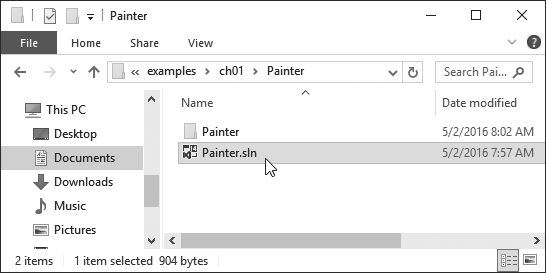
\includegraphics[width=\textwidth,height=0.75\textheight,keepaspectratio]{images/fig1_8_painter_solution.png}\\
      \scriptsize \color{gray} Hình 1.8: Cấu trúc thư mục ứng dụng Painter và tệp Painter.sln (Deitel p.64)
    \end{column}
  \end{columns}
\end{frame}

% ==============================================================================
% SLIDE 37: 1.12 CASE STUDY: ỨNG DỤNG PAINTER
% ==============================================================================
\begin{frame}{1.12 Case Study: Ứng dụng Đồ họa Painter (Visual C\# GUI)}
  \begin{columns}[c]
    \begin{column}{0.50\textwidth}
      \begin{block}{\textbf{Mô tả Ứng dụng Painter (Deitel Section 1.12):}}
        \begin{itemize}
          \item Một ứng dụng vẽ hình đồ họa Windows Forms trực quan hoàn chỉnh.
          \item Người dùng chọn màu cọ vẽ: \textbf{Red, Blue, Green, Black}.
          \item Người dùng chọn kích thước cọ: \textbf{Small, Medium, Large}.
          \item Di chuột trên vùng vẽ màu trắng (\textbf{Panel}) để tạo các bức tranh nghệ thuật.
          \item Cung cấp nút \textbf{Undo} (hoàn tác) và \textbf{Clear} (xóa sạch vẽ lại).
        \end{itemize}
      \end{block}
    \end{column}
    \begin{column}{0.48\textwidth}
      \begin{tcolorbox}[colback=UniLightBlue,colframe=UniBlue,title=\textbf{Bài học Sư phạm cốt lõi}]
        \begin{itemize}\scriptsize
          \item Giúp sinh viên thấy ngay thành quả trực quan sống động của lập trình C\# ngay trong buổi học đầu tiên!
          \item Không cần viết hàng trăm dòng code đồ họa phức tạp từ đầu; tận dụng các điều khiển GUI có sẵn trong .NET Framework.
        \end{itemize}
      \end{tcolorbox}
    \end{column}
  \end{columns}
\end{frame}

% ==============================================================================
% SLIDE 38: KHẢO SÁT CÁC ĐIỀU KHIỂN GUI TRONG PAINTER
% ==============================================================================
\begin{frame}{Khảo sát các Điều khiển Đồ họa GUI (Hình 1.10)}
  \begin{columns}[c]
    \begin{column}{0.52\textwidth}
      \centering
      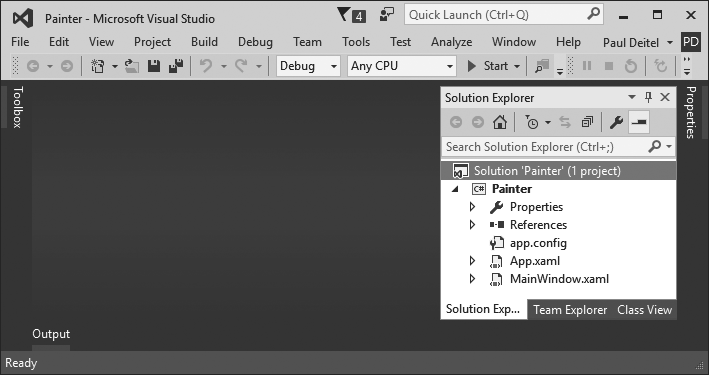
\includegraphics[width=\textwidth,height=0.78\textheight,keepaspectratio]{images/fig1_10_painter_app_gui.png}\\
      \scriptsize \color{gray} Hình 1.10: Các thành phần điều khiển GUI trong ứng dụng Painter (Deitel p.65)
    \end{column}
    \begin{column}{0.46\textwidth}
      \begin{block}{\textbf{4 Loại Điều khiển GUI chính:}}
        \begin{enumerate}\scriptsize
          \item \textbf{GroupBox:} Khung viền nhóm các điều khiển có liên quan với nhau về mặt ngữ nghĩa (nhóm Color, nhóm Size).
          \item \textbf{RadioButton:} Nút chọn tròn độc quyền; trong cùng 1 GroupBox, chỉ có \textbf{duy nhất 1 nút} được chọn tại một thời điểm.
          \item \textbf{Panel:} Vùng không gian nền trắng tiếp nhận thao tác vẽ và tọa độ chuột.
          \item \textbf{Button:} Nút bấm kích hoạt hành động tức thì (\texttt{Undo}, \texttt{Clear}).
        \end{enumerate}
      \end{block}
    \end{column}
  \end{columns}
\end{frame}

% ==============================================================================
% SLIDE 39: LẬP TRÌNH HƯỚNG SỰ KIỆN (EVENT-DRIVEN) TRONG GUI
% ==============================================================================
\begin{frame}{Cơ chế Lập trình Hướng sự kiện (Event-Driven Mechanism)}
  \begin{columns}[T]
    \begin{column}{0.48\textwidth}
      \begin{block}{\textbf{Mô hình Hướng sự kiện hoạt động thế nào?}}
        \begin{itemize}
          \item Ứng dụng không chạy tuần tự từ dòng đầu đến dòng cuối rồi thoát.
          \item Ứng dụng rơi vào trạng thái \textbf{"Lắng nghe" (Event Loop)}, kiên nhẫn chờ đợi tương tác từ người dùng.
          \item Khi người dùng tương tác $\to$ Hệ điều hành gửi thông điệp sự kiện $\to$ Phương thức xử lý sự kiện (\textbf{Event Handler}) tương ứng được kích hoạt.
        \end{itemize}
      \end{block}
    \end{column}
    \begin{column}{0.48\textwidth}
      \begin{tcolorbox}[colback=CSharpPurple!5,colframe=CSharpPurple,title=\textbf{Các sự kiện trong Ứng dụng Painter}]
        \begin{itemize}\scriptsize
          \item \texttt{RadioButton.CheckedChanged}: Đổi màu hoặc kích thước cọ vẽ ngay khi người dùng chọn.
          \item \texttt{Panel.MouseDown}: Nhận biết người dùng bắt đầu nhấn chuột xuống bề mặt vẽ.
          \item \texttt{Panel.MouseMove}: Bắt tọa độ $(X, Y)$ liên tục khi rê chuột để vẽ các hình tròn màu.
          \item \texttt{Button.Click}: Xử lý xóa tranh (\texttt{Clear}) hoặc quay lại nét trước (\texttt{Undo}).
        \end{itemize}
      \end{tcolorbox}
    \end{column}
  \end{columns}
\end{frame}

% ==============================================================================
% SLIDE 40: [HANDS-ON LAB 3] TEST-DRIVE PAINTER APP
% ==============================================================================
\begin{frame}{[HANDS-ON LAB 3] Test-Drive Ứng dụng Painter tại Lớp IT26M}
  \begin{block}{\textbf{Thực hành Chạy thử \& Tương tác 3 Bước (20 Phút tại phòng máy):}}
  \end{block}
  \begin{columns}[T]
    \begin{column}{0.32\textwidth}
      \centering
      \textbf{\scriptsize Bước 1: Vẽ cánh hoa (Red / Small)}\\
      \vskip 1mm
      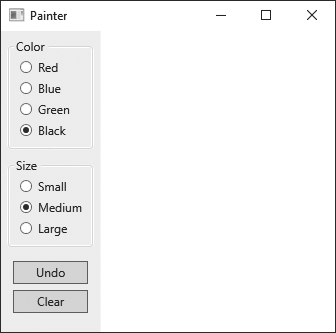
\includegraphics[width=\textwidth,height=0.45\textheight,keepaspectratio]{images/fig1_11_drawing_petals.png}\\
      \vskip 1mm
      \scriptsize \color{gray} Chọn Red + Small, vẽ các cánh hoa tròn uốn lượn (Hình 1.11)
    \end{column}
    \begin{column}{0.32\textwidth}
      \centering
      \textbf{\scriptsize Bước 2: Vẽ cành \& cỏ (Green / Large)}\\
      \vskip 1mm
      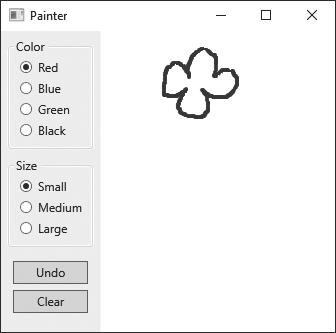
\includegraphics[width=\textwidth,height=0.45\textheight,keepaspectratio]{images/fig1_12_drawing_stem_grass.png}\\
      \vskip 1mm
      \scriptsize \color{gray} Chọn Green + Large, kéo thẳng vẽ thân hoa và thảm cỏ xanh (Hình 1.12)
    \end{column}
    \begin{column}{0.32\textwidth}
      \centering
      \textbf{\scriptsize Bước 3: Vẽ hạt mưa (Blue / Medium)}\\
      \vskip 1mm
      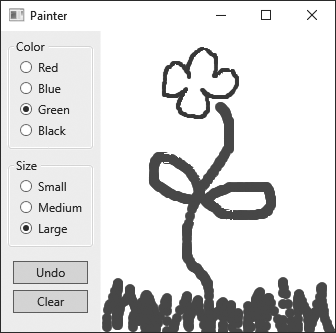
\includegraphics[width=\textwidth,height=0.45\textheight,keepaspectratio]{images/fig1_13_drawing_complete.png}\\
      \vskip 1mm
      \scriptsize \color{gray} Chọn Blue + Medium, chấm các hạt mưa hoàn tất bức tranh (Hình 1.13)
    \end{column}
  \end{columns}
\end{frame}

% ==============================================================================
% SLIDE 41: [CHECKPOINT 3] TRẮC NGHIỆM TIẾT 3
% ==============================================================================
\begin{frame}{[CHECKPOINT 3] Kiểm tra Nhanh Kiến thức Tiết 3}
  \begin{tcolorbox}[colback=UniOrange!5,colframe=UniOrange,top=1.5mm,bottom=1.5mm,title=\textbf{Câu hỏi 1: Trong ứng dụng Painter, điều khiển nào chứa vùng vẽ màu trắng?}]
    \begin{itemize}\scriptsize
      \item[A.] GroupBox
      \item[B.] RadioButton
      \item[C.] \textbf{Panel} \hfill \textit{\color{UniGreen}\textbf{[ĐÁP ÁN ĐÚNG]}}
      \item[D.] Button
    \end{itemize}
  \end{tcolorbox}
  \vskip 1mm
  \begin{tcolorbox}[colback=UniNavy!5,colframe=UniNavy,top=1.5mm,bottom=1.5mm,title=\textbf{Câu hỏi 2: Phím tắt chuẩn trong Visual Studio để biên dịch và chạy ứng dụng là gì?}]
    \begin{itemize}\scriptsize
      \item[A.] F1
      \item[B.] \textbf{F5 (hoặc Ctrl + F5 để chạy không debug)} \hfill \textit{\color{UniGreen}\textbf{[ĐÁP ÁN ĐÚNG]}}
      \item[C.] F12
      \item[D.] Ctrl + S
    \end{itemize}
  \end{tcolorbox}
\end{frame}

% ==============================================================================
% SLIDE 42: TỔNG KẾT TOÀN DIỆN CHƯƠNG 1
% ==============================================================================
\begin{frame}{Tổng kết Toàn diện Chương 1: Checklist Chuẩn Đầu Ra}
  \begin{exampleblock}{\textbf{Chúc mừng sinh viên lớp IT26M đã hoàn thành trọn vẹn 5 Chuẩn đầu ra:}}
    \begin{itemize}
      \item[$\checkmark$] \textbf{CLO 1.1:} Nắm chắc cấu trúc 6 khối logic máy tính và bảng phân cấp dữ liệu từ Bit $\to$ Big Data.
      \item[$\checkmark$] \textbf{CLO 1.2:} Phân biệt Compiler vs Interpreter; thấu hiểu bản chất Công nghệ Đối tượng (Class vs Object, Đóng gói, Kế thừa).
      \item[$\checkmark$] \textbf{CLO 1.3:} Giải thích thông suốt cơ chế thực thi .NET: Mã nguồn C\# $\to$ MSIL $\to$ CLR JIT $\to$ Native Machine Code; hiểu lợi thế của Managed Code.
      \item[$\checkmark$] \textbf{CLO 1.4:} Làm chủ môi trường Visual Studio IDE (Solution, Project, Form Designer, Toolbox, Properties).
      \item[$\checkmark$] \textbf{CLO 1.5:} Trải nghiệm thành công mô hình Lập trình trực quan và Hướng sự kiện qua Case Study Painter App.
    \end{itemize}
  \end{exampleblock}
\end{frame}

% ==============================================================================
% SLIDE 43: NHIỆM VỤ TỰ HỌC & BÀI TẬP VỀ NHÀ
% ==============================================================================
\begin{frame}{Nhiệm vụ Tự học \& Chuẩn bị cho Buổi học tiếp theo}
  \begin{columns}[T]
    \begin{column}{0.48\textwidth}
      \begin{block}{\textbf{Bài tập về nhà (Chương 1):}}
        \begin{enumerate}
          \item Đọc kỹ toàn bộ Chapter 1 trong giáo trình \textit{Visual C\# How to Program} (trang 41 -- 72).
          \item Hoàn thành các câu hỏi \textbf{Self-Review Exercises} 1.1 đến 1.29 cuối chương.
          \item Tự cài đặt \textbf{Visual Studio 2022 Community} (miễn phí) trên laptop cá nhân với workload \textit{".NET desktop development"}.
        \end{enumerate}
      \end{block}
    \end{column}
    \begin{column}{0.48\textwidth}
      \begin{tcolorbox}[colback=CSharpPurple!10,colframe=CSharpPurple,title=\textbf{Đọc trước Chương 2: Nhập môn Cú pháp C\#}]
        \begin{itemize}
          \item Viết ứng dụng C\# Console đầu tiên: \texttt{Console.WriteLine}.
          \item Cú pháp hàm \texttt{Main}, quy ước đặt tên định danh, chú thích mã nguồn.
          \item Nhập xuất dữ liệu với \texttt{Console.ReadLine}.
          \item Kiểu dữ liệu nguyên thủy, toán tử số học và cấu trúc rẽ nhánh cơ bản (\texttt{if}).
        \end{itemize}
      \end{tcolorbox}
    \end{column}
  \end{columns}
\end{frame}

% ==============================================================================
% SLIDE 44: LỜI CẢM ƠN
% ==============================================================================
\begin{frame}[plain]
  \vfill
  \centering
  \begin{beamercolorbox}[sep=8pt,center,shadow=true,rounded=true]{palette primary}
    \usebeamerfont{title}\Huge \textbf{CẢM ƠN CÁC BẠN SINH VIÊN}\\[2mm]
    \Huge \textbf{LỚP IT26M!}\\[4mm]
    \large \textbf{CHÚC CÁC BẠN HỌC TẬP TỐT VÀ LÀM CHỦ CÔNG NGHỆ C\# \& .NET}
  \end{beamercolorbox}
  \vskip 6mm
  \begin{beamercolorbox}[sep=4pt,center]{palette secondary}
    \small \textbf{Hỏi đáp \& Thảo luận trực tiếp tại giảng đường / Diễn đàn LMS môn học}
  \end{beamercolorbox}
  \vfill
\end{frame}

\end{document}
